\chapter{Search for invisibly decaying Higgs bosons in Run 1 parked data}
\label{chap:parked}
The parked data, described in \SectionRef{sec:triggers}, used for this analysis was collected using a range of triggers with similar but looser requirements than that used for the prompt data analysis described in the previous chapter. These looser requirements allow areas of phase space which were previously removed by the prompt trigger to be used. However, these regions also have very high levels of \ac{QCD} multijet backgrounds, and require the analysis selection and some background estimation methods to be redesigned compared to the prompt analysis.

%??prkedgains111114.pdf for parked vs prompt limits
%??closure161214update for closure test
%??invupdate081214.pdf for some pileup studies
%??framework synch fwprogress300614.pdf
%??preapproval for source of gain and other good things
%??As above for prompt data analysis but focus on differences and limit setting:
%??New trigger efficiency characterisation, systematic improvements, signal region optimisation, differences in background estimations including options not used
%??lepton and jet pt requirements
\section{Trigger}
\label{sec:parkedtrigger}
The parked data trigger varied throughout LHC Run 1. Run 1 was split into 4 ``eras'', A, B, C and D. During era A data was not being parked, so the prompt data is used. The two other triggers used, one for eras B and C, and one for era D, differed from the prompt trigger in that there was no requirement on the \MET present in each event and the jet \pt and \Mjj requirements were looser. The exact values of the trigger selection cuts are summarised in \TableRef{tab:parkedtrig}.

\begin{table}
  \caption{A summary of the requirements of the triggers used for this analysis in each of LHC Run 1's eras. For the jet requirements all triggers require that there is at least one pair of jets in the event satisfying all of the jet requirements listed in this table. All requirements are on \ac{HLT} variables unless stated otherwise.}
  \label{tab:parkedtrig}
  \begin{tabular}{lc|c|c}
    \hline\hline
    \multirow{2}{*}{Variable} & \multicolumn{3}{c}{Cut in era} \\
    \cline{2-4}
    & A & B \& C & D \\
    \hhline{====}
    L1 \MET & \multicolumn{3}{c}{$>40$ \GeV} \\
    \hline
    \METnoMU & $>65$ \GeV & \multicolumn{2}{c}{No requirement} \\
    \hline
    jet \pt of both jets & $>40$ \GeV & $>35$ \GeV & $>30$ \GeV \\
    \hline
    \Mjj & $>800$ \GeV & \multicolumn{2}{c}{$>700$ \GeV} \\
    \hline
    \detajj & \multicolumn{3}{c}{$>3.5$} \\
    \hline
    $\eta_{j1}\cdot\eta_{j2}$ & \multicolumn{3}{c}{$>0$} \\
    \hline
    \hline
  \end{tabular}
\end{table}

As three different triggers are used the measurement of trigger efficiency must be performed separately for each one. Also, the variables used in the trigger are highly correlated with each other. These correlations mean it is important to either only use regions of phase space where the trigger is fully efficient, as was done in the prompt analysis, or to measure the trigger efficiency in a way that accurately models the effect of these correlations. The cuts required to ensure that each trigger is fully efficient throughout the region selected can be ascertained from \FigureRef{fig:prompttrigplots}. As the trigger used in era A was the same as that used for the prompt analysis, no relaxation would be possible if the data from era A is to be used. Era A only accounts for 5\% of the total data, however even if the analysis selection was chosen such that only the loosest trigger is fully efficient the common \ac{L1} \MET requirements in all three triggers mean that only the thresholds on the sub-leading jet's \pt and the \Mjj would be able to be relaxed and it would still be necessary to discard data in the trigger turn on region which is expected to contain signal events. For these reasons several approaches to measuring the trigger efficiency as a function of the values of all variables used in it were investigated.

First, the trigger efficiency was measured three dimensionally as a function of \METnoMU, \Mjj and sub-leading jet's \pt. An example of one of the results of these mearements in one of the bins in \METnoMU for the era B and C, and the era D triggers can be seen in \FigureRef{fig:parked3dtrigeff}. The three variables used were chosen, as the trigger becomes fully efficient very quickly as a function of the $\eta$ related variables, so no parametrisation of the efficiency is necessary. The number and size of the bins was chosen to ensure that sufficient events are present in each bin to prevent the statistical error on the efficiency measurement being larger than the differences between bins. As can be seen from the figure, this leads to very large differences in efficiency between bins, which leads to discontinuities in the \METnoMU, \Mjj and sub-leading jet \pt distributions when the measured efficiency was applied to \ac{MC} events as a weight. This method was therefore not suitable for use in the final analysis.
%trigeff070414.pdf for full 3D binned plot
\begin{figure} 
  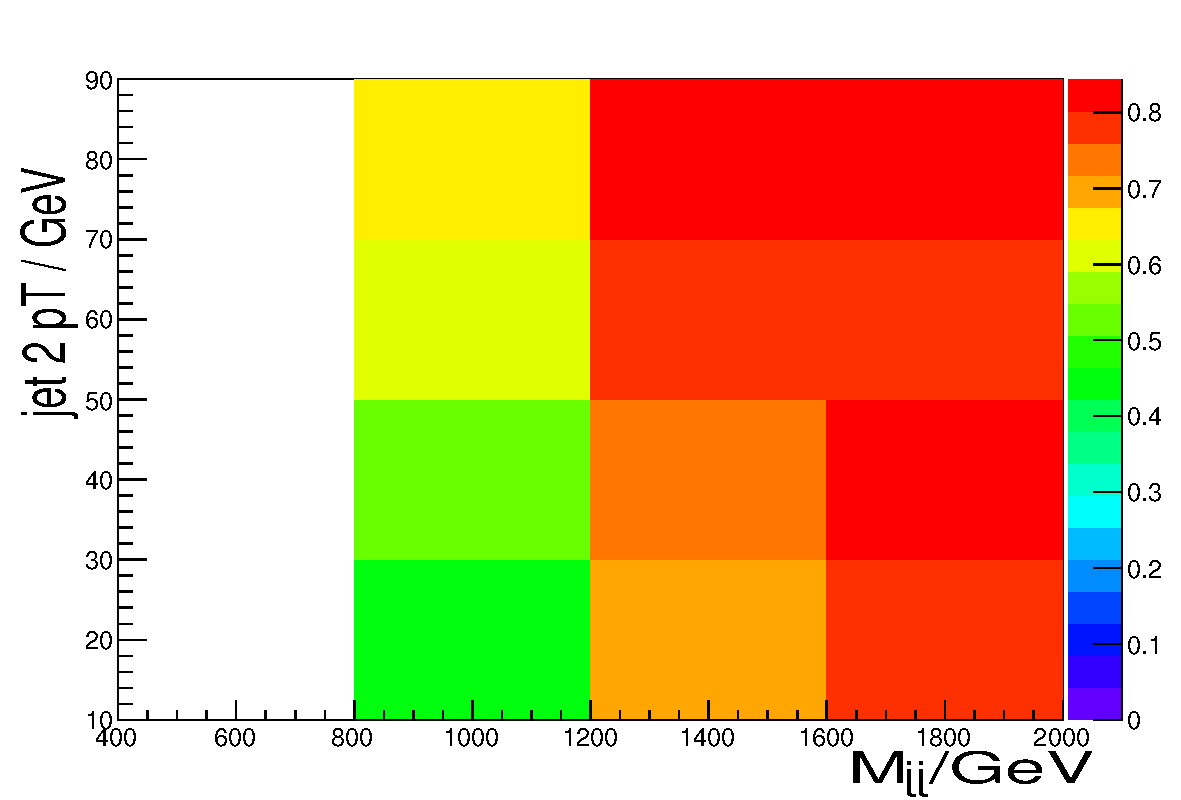
\includegraphics[width=.6\largefigwidth]{plots/parked/HLT_DiJet35_MJJ700_AllJets_DEta3p5_VBFmet120trigeff.pdf}
  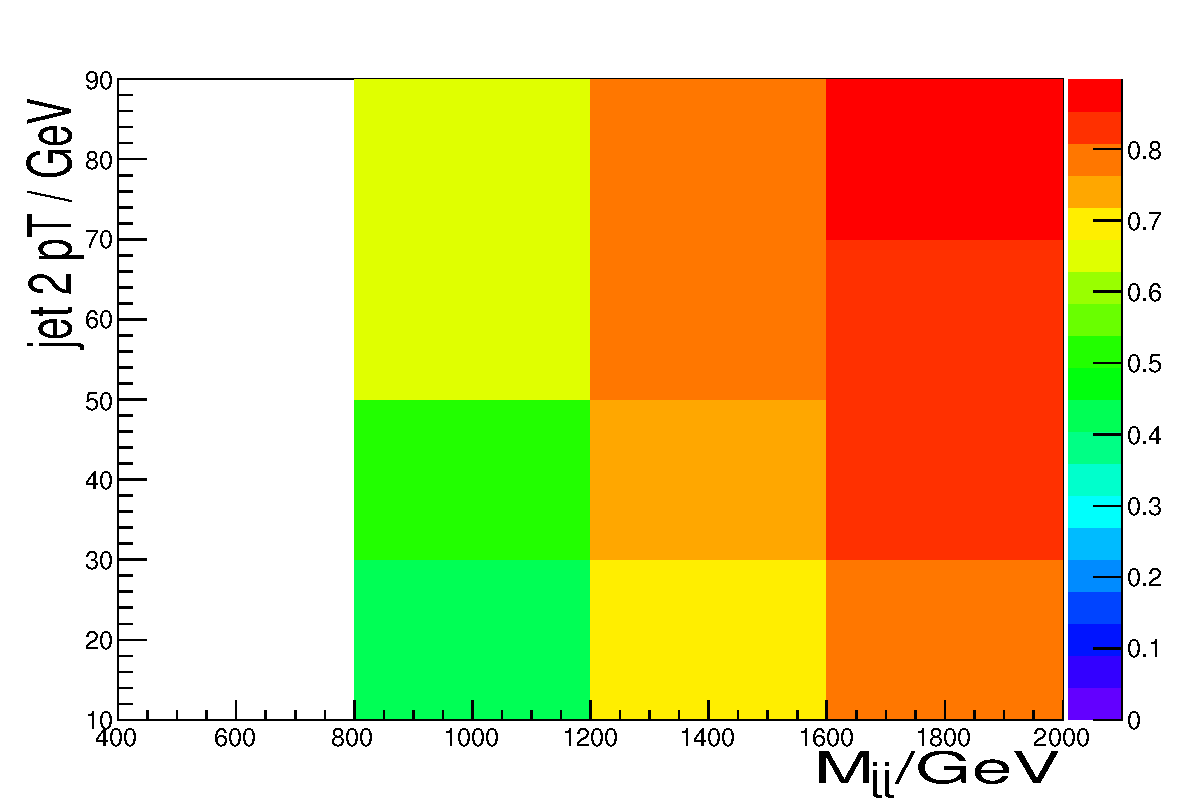
\includegraphics[width=.6\largefigwidth]{plots/parked/HLT_DiJet30_MJJ700_AllJets_DEta3p5_VBFmet120trigeff.pdf}
 \caption{The efficiency for the trigger (color-scale) used in eras B and C (left) and era D (right), as a function of \Mjj and sub-leading jet \pt for events with \METnoMU between 60 and 120 \GeV. The efficiency was measured using a single muon dataset collected with an orthogonal trigger.}
  \label{fig:parked3dtrigeff}
\end{figure}

In order to achieve a smoother trigger efficiency parametrisation, coarse bins in \Mjj and sub-leading jet \pt were chosen and a fit to the \METnoMU efficiency distribution in each bin was performed, using the following function:
\begin{equation}
  \label{eq:parkedtrigfunc}
  f\left(x\right)=\frac{A}{2}\cdot\left(1+ \frac{2}{\sqrt{\pi}}\int_{0}^{\frac{x-B}{\sqrt{C}}}e^{-t^{2}}\mathrm{d}t\right),
\end{equation}
which has a maximum value of A, and is derived from the error function with centre B and width C. The width, maximum and centre of the function are all allowed to float in the fit. The events used in this study were required to have leading jet \pt$>50$ \GeV, $\eta_{j1}\cdot\eta_{j2}<0$ and \detajj$>3.6$ to ensure that there are no inefficiencies due to these variables. The results of these fits for two representative \Mjj and sub-leading jet \pt bins are shown in \FigureRef{fig:parkedtrigeff}, and the results for the remaining bins are shown in \AppendixRef{app:trigeffs}. Some of the plots in the appendix indicate that the parameters of the fit have taken extreme values, or have very large uncertainties. These extreme values and poor fits are mostly due to low numbers of events in the bin, and as described in \SectionRef{sec:parkedsel}, these bins are not used in the final event selection.

\begin{figure}
  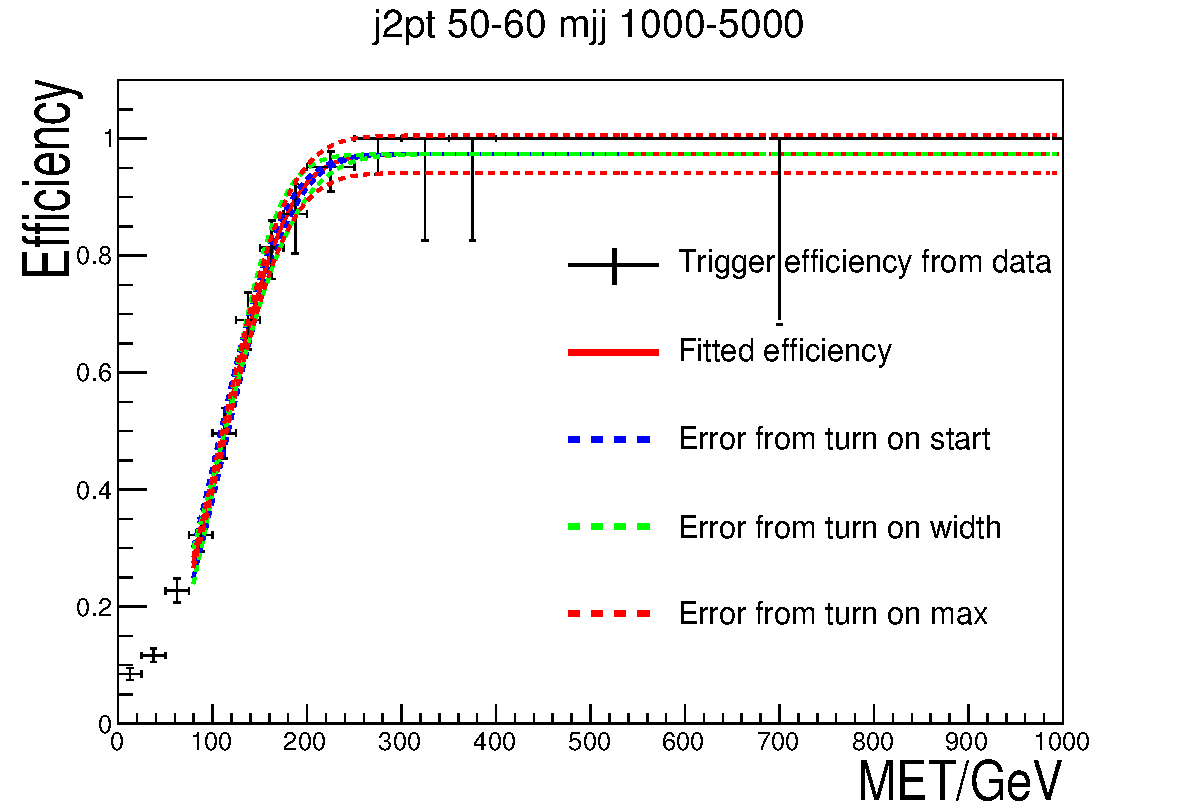
\includegraphics[width=.6\largefigwidth]{plots/parked/trigfitplots/hData_MET_1D_35D.pdf}
  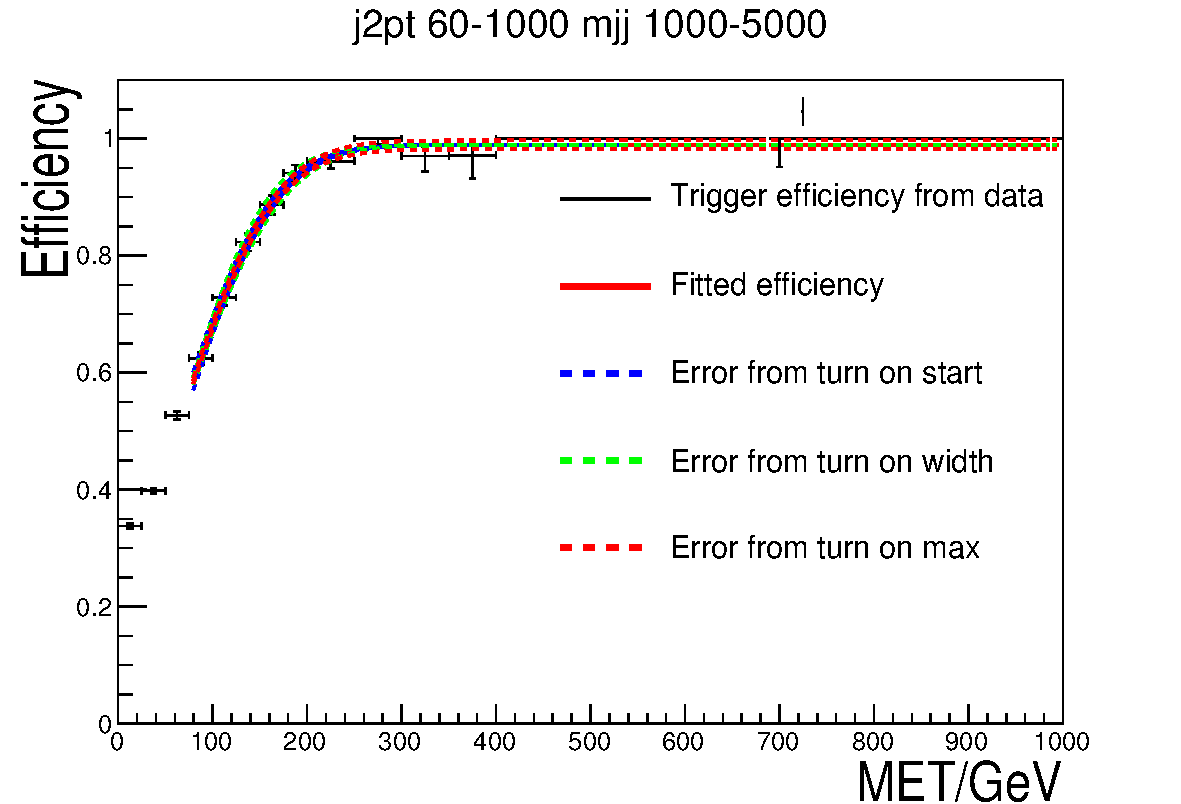
\includegraphics[width=.6\largefigwidth]{plots/parked/trigfitplots/hData_MET_1D_45D.pdf}
  \caption{The results of performing a fit of the function in \EquationRef{eq:parkedtrigfunc} to the efficiency of the trigger used in era D, measured in a sample of single muon events collected with an orthogonal trigger. The dashed bands show the uncertainty on the fit due to each of the three parameters of the fit. The two bins of dijet mass (mjj) and sub-leading jet's \pt (j2pt) shown are those with the two highest numbers of events from the final signal region described in \SectionRef{sec:parkedsel}.}
  \label{fig:parkedtrigeff}
\end{figure}

 The weight applied to each \ac{MC} event is an average of the efficiency found for each of the three triggers weighted as follows by the amount of integrated luminosity recorded using each trigger:
\begin{equation}
  \label{eq:parkedtrigweight}
  w\left(p_{\mathrm{T}j2},\Mjj,\METnoMU\right)=\frac{\sum_{i}\mathcal{L}_{i}\epsilon_{i}\left(p_{\mathrm{T}j2},\Mjj,\METnoMU\right)}{\sum_{i}\mathcal{L}_{i}},
\end{equation}
Where $i$ are the three triggers, $\epsilon_{i}\left(p_{\mathrm{T}j2},\Mjj,\METnoMU\right)$ is the measured efficiency for trigger $i$ as a function of the event's sub-leading jet \pt, \Mjj and \METnoMU, and $\mathcal{L}_{i}$ is the integrated luminosity collected using trigger $i$. The resulting trigger efficiency varies smoothly and leads to no unphysical discontinuities in the distributions of event variables as can be seen from the figures in the remainder of this chapter.

\section{Event selection}
\label{sec:parkedsel}
As mentioned above a significant challenge of the parked data analysis is that the areas of phase space collected by the parked data triggers but not by the prompt data triggers have very large contributions from \ac{QCD} multijet backgrounds. The \ac{QCD} multijet contribution to \ac{VBF} analyses is very hard to model because whilst the cross-sections for these processes are very high, the probability of any individual event being \ac{VBF}-like is very low, making the number of \ac{MC} events that must be generated prohibitively large. As a result of these difficulties the parked data selection is separated into two stages. The first ``preselection'' stage selects a region of phase space which is not expected to be dominated by \ac{QCD} processes. After this preselection has been made the background processes expected to make contributions are the same as in the prompt data analysis, and studies were undertaken into which background estimation methods and final signal region selection led to the best expected limit.

%??runcbug101114.pdf sig reg optimisation

\subsection{Preselection}
\label{sec:parkedpresel}
The first element of the preselection was motivated by the trigger. The following selection was applied to ensure that the values of all event variables are above the trigger thresholds of all triggers used:
\begin{align}
  \label{eq:parkedprepresel}
  \begin{split}
  \eta_{j1}\cdot\eta_{j2}<0,\,\mathrm{leading\,jet\,}\pt>50 \GeV, \detajj>3.6, \\
  \mathrm{subleading\,jet\,}\pt>40 \GeV, \Mjj>800 GeV, \METnoMU>90\GeV.
  \end{split}
\end{align}
Where $j1$ and $j2$ are the leading and sub-leading \pt jets in the event and are chosen as the \ac{VBF} tag jets. We also require that for the ``signal-like'' selection there are no veto electrons or muons in the event. the W+jets and Z+jets control regions used in the background estimation methods described in \SectionRef{sec:parkedbkg} impose different lepton requirements. QCD multijet processes still dominate the region defined by this selection, as can be seen in \FigureRef{fig:parkedpresel} top left, where there are a lot more data events than expected from the background \ac{MC} prediction. This difference is due to mismeasured \ac{QCD} multijets events not being adequately modelled by the available \ac{MC} samples. Further pre-selection was therefore necessary to reduce the mismeasured \ac{QCD} multijet background to a level where the large uncertainties on any estimation of its contribution do not have a significant effect on the analysis.

The first variable that was used to achieve this reduction is the \MET significance, \METsig, which is defined as the ratio between \METnoMU and the square root of the sum of the transverse energy of all particles in the event which is an estimate of the statistical error on the \MET. The preselection requires that this variable be greater than 3. The value of this cut was chosen by looking at \FigureRef{fig:parkedpresel} top left and removing the region with the most disagreement between data and \ac{MC}. The resulting region shown in \FigureRef{fig:parkedpresel} top right still does not display good agreement between data and the \ac{MC} prediction, however the disagreement is smaller.

After the cut on \METsig, a requirement that the \METnoMU is not too close to any jets in \phi was made. This requirement was motivated by the high probability for the \MET to be aligned with jets that have been mismeasured. Two variables were investigated, the first was the minimum azimuthal angle difference between either of the two tag jets and the \METnoMU, \jetmetdphileading, and the second was the minimum azimuthal angle difference between any jet with \pt greater than 30 \GeV and the \METnoMU, \jetmetdphi. At a similar signal efficiency the difference between the observed number of events and the \ac{MC} background prediction, which is an indication of the remaining \ac{QCD} multijet background, was found to be 80\% smaller for a cut on \jetmetdphi than a cut on \jetmetdphileading. The same cut on \jetmetdphi was also found to reduce top quark related backgrounds by a factor of two compared to a cut on \jetmetdphileading. We therefore require that \jetmetdphi$>1.0$ for events to pass the preselection. \jetmetdphi was found to give significantly better signal efficiency than \dphijj for the same background rejection, so no cut was made on \dphijj.

%AN-14-243
\begin{figure}
  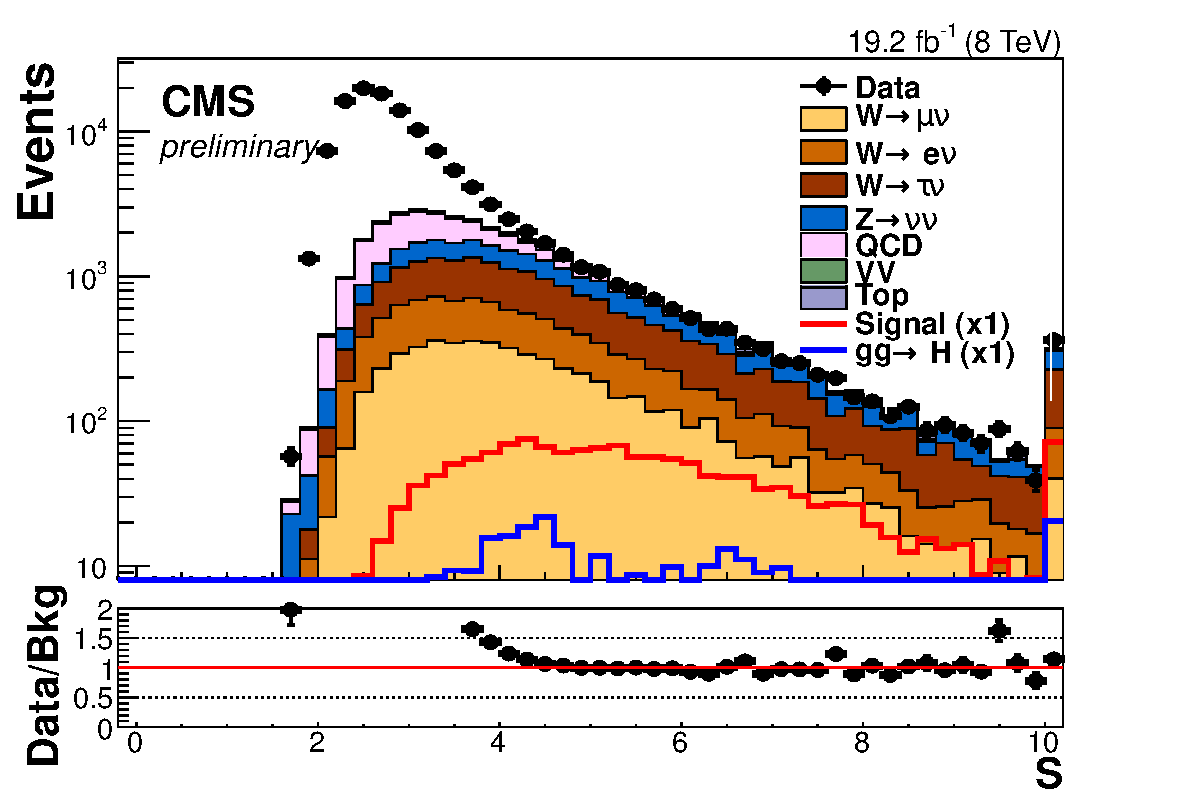
\includegraphics[width=.6\largefigwidth]{plots/parked/AN-14-243-figs/lognopreselnunu_metnomu_significance.pdf}
  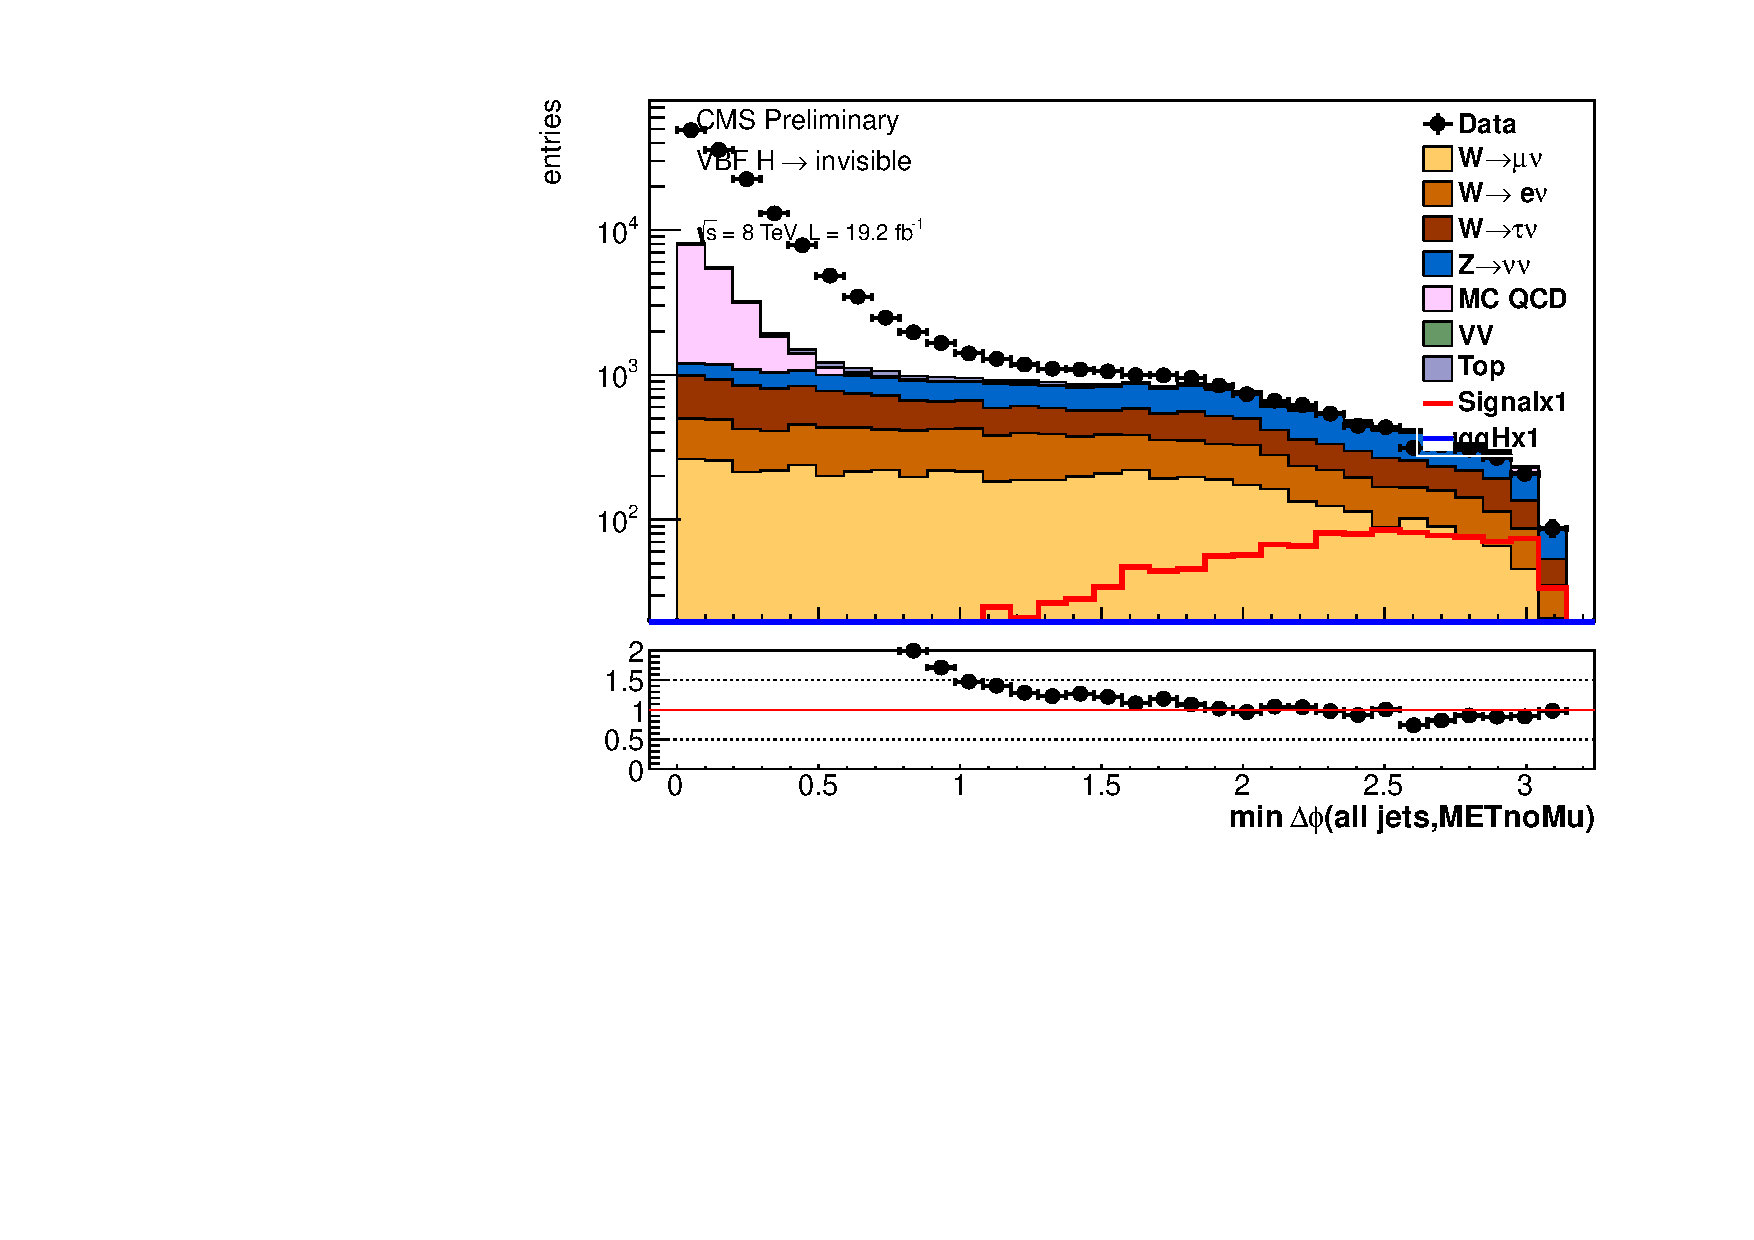
\includegraphics[width=.6\largefigwidth]{plots/parked/AN-14-243-figs/logmetsigpreselnunu_alljetsmetnomu_mindphi.pdf}

  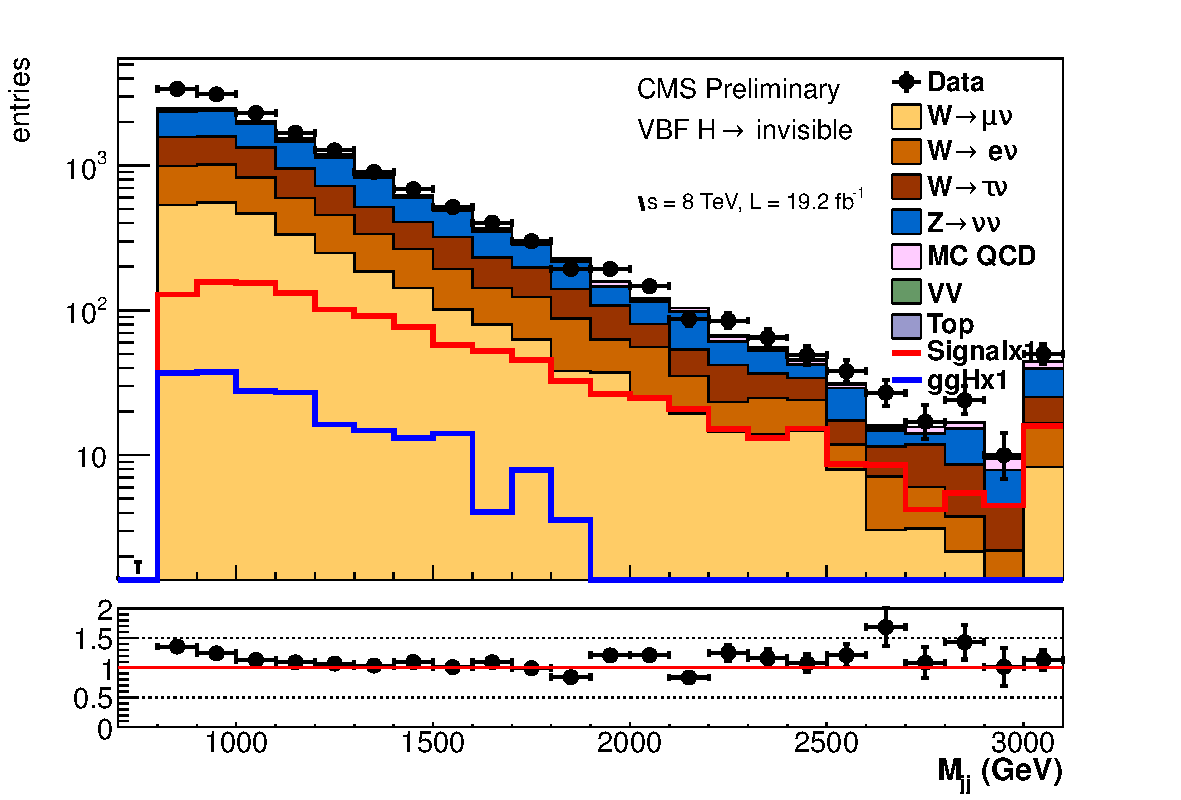
\includegraphics[width=.6\largefigwidth]{plots/parked/AN-14-243-figs/logmjj800nunu_dijet_M.pdf}
  \caption{Top left: \METsig after the trigger driven selection described in \EquationRef{eq:parkedprepresel}. Top right: \jetmetdphi after the trigger driven selection and requiring \METsig$>3$. Bottom: \Mjj after the trigger driven selection and requiring \METsig$>3$ and \jetmetdphi$>1$. All three plots are of the signal-like region with the \ac{MC} scaled using the background estimation methods described in \SectionRef{sec:parkedbkg}. The disagreement between data and the predictions from background \ac{MC} samples is believed to be due to mismeasured \ac{QCD} multijet events which are not well moddelled by the available \ac{MC} samples.}
  \label{fig:parkedpresel}
\end{figure}

%contplotsandpresel160914
The \Mjj distribution after the \jetmetdphi cut is shown in \FigureRef{fig:parkedpresel} bottom. Whilst the agreement for large \Mjj is good, it can be seen that the first bin of the distribution, where mismeasured \ac{QCD} multijet events would be expected, due to their not recoiling against another object, shows a significant disagreement. The final cut of the preselection is therefore to require that \Mjj$>1000$ \GeV. In summary the full preselection is as follows:
\begin{equation}
  \label{eq:presel}
  \begin{split}
  \eta_{j1}\cdot\eta_{j2}<0,\,\mathrm{leading\,jet\,}\pt>50 \GeV, \detajj>3.6, \\
  \mathrm{subleading\,jet\,}\pt>40 \GeV, \Mjj>1000 GeV, \METnoMU>90\GeV, \\
  \jetmetdphi>1.0, \METsig>3.0.
  \end{split}
\end{equation}
Distributions of several variables after the full preselection are shown in \FigureRef{fig:parkedpostpresel}.

\begin{figure}
  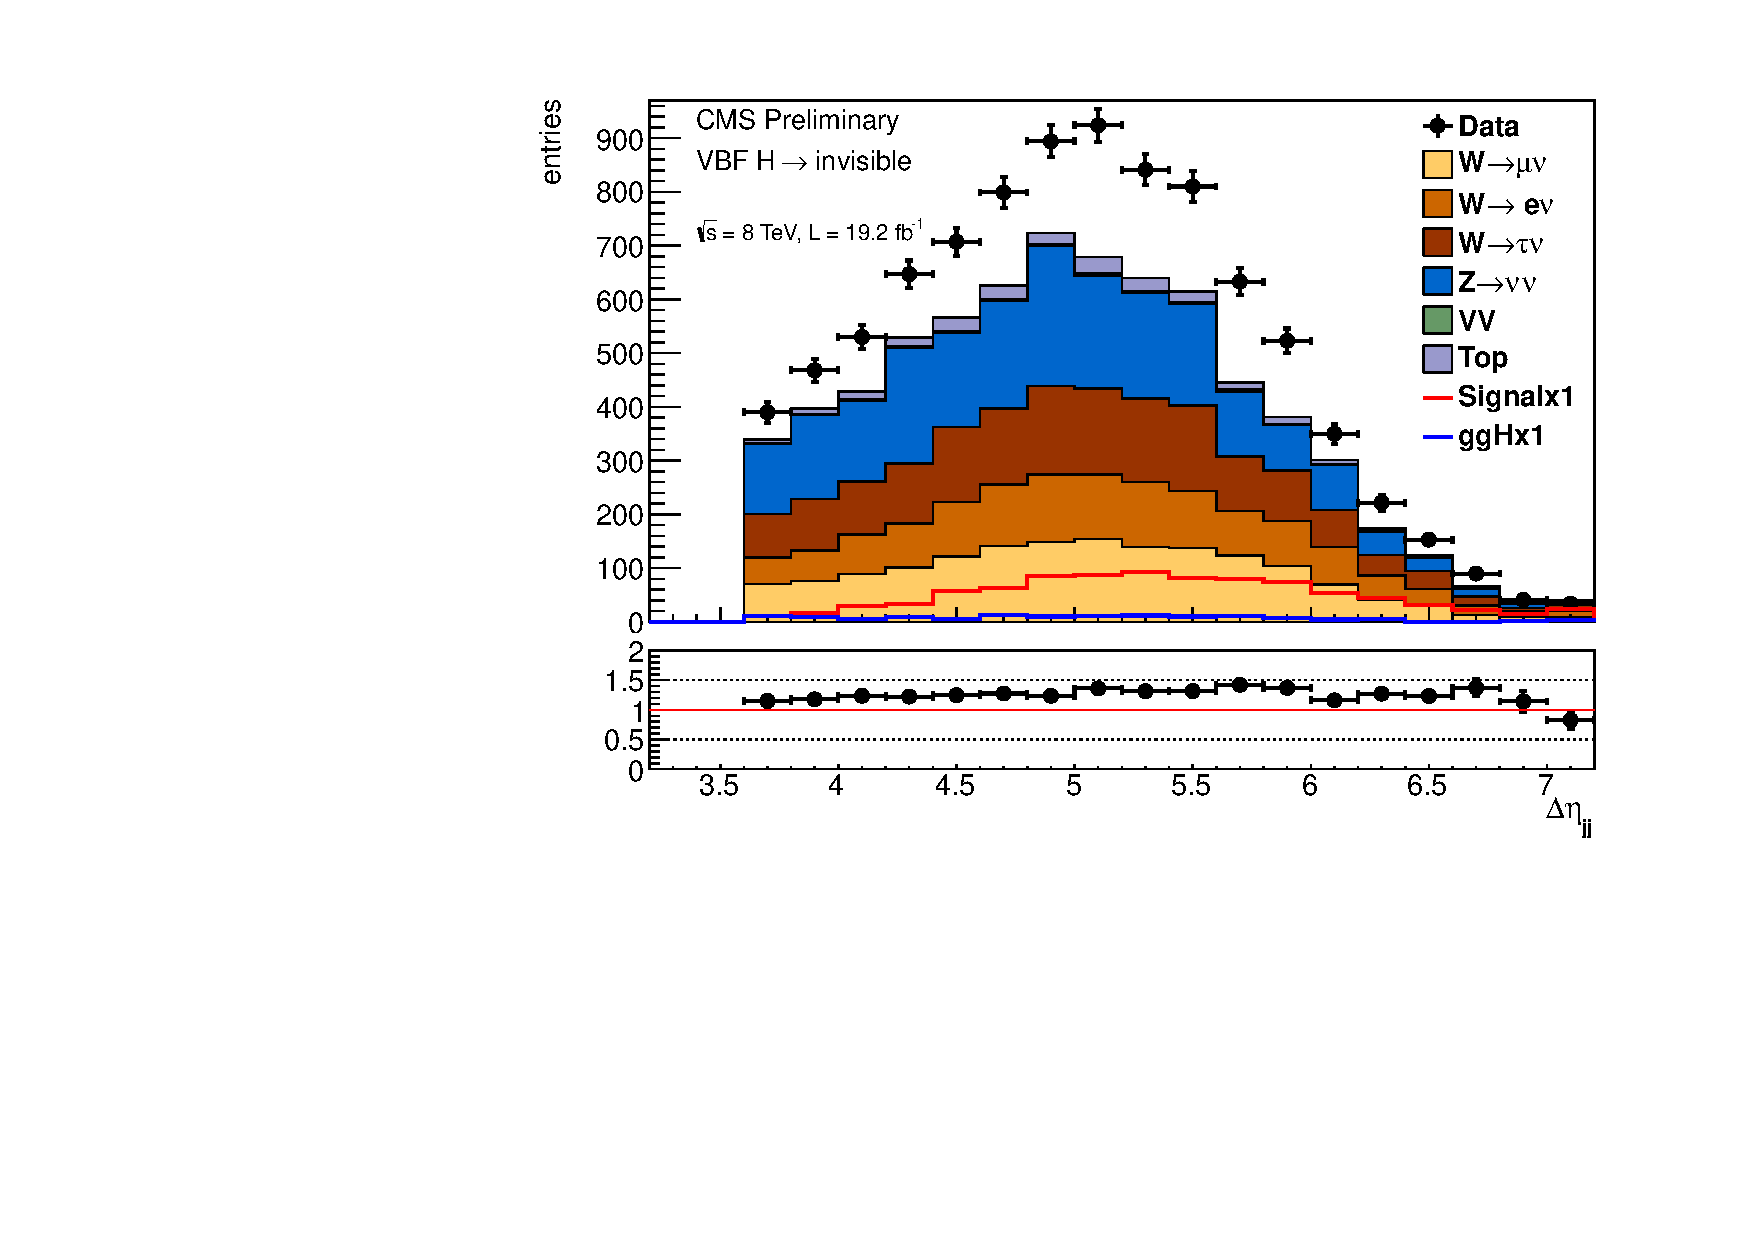
\includegraphics[width=.6\largefigwidth]{plots/parked/AN-14-243-figs/output_presel/nunu_dijet_deta.pdf}
    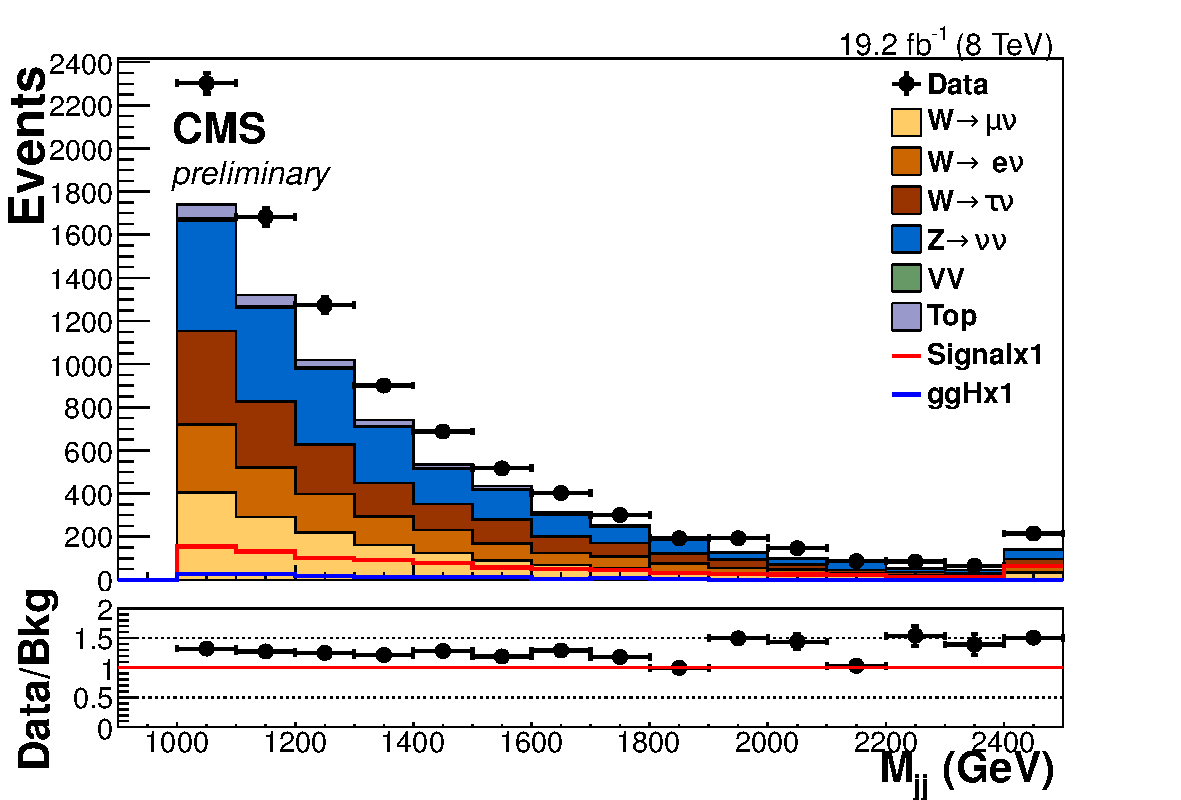
\includegraphics[width=.6\largefigwidth]{plots/parked/AN-14-243-figs/output_presel/nunu_dijet_M.pdf}

    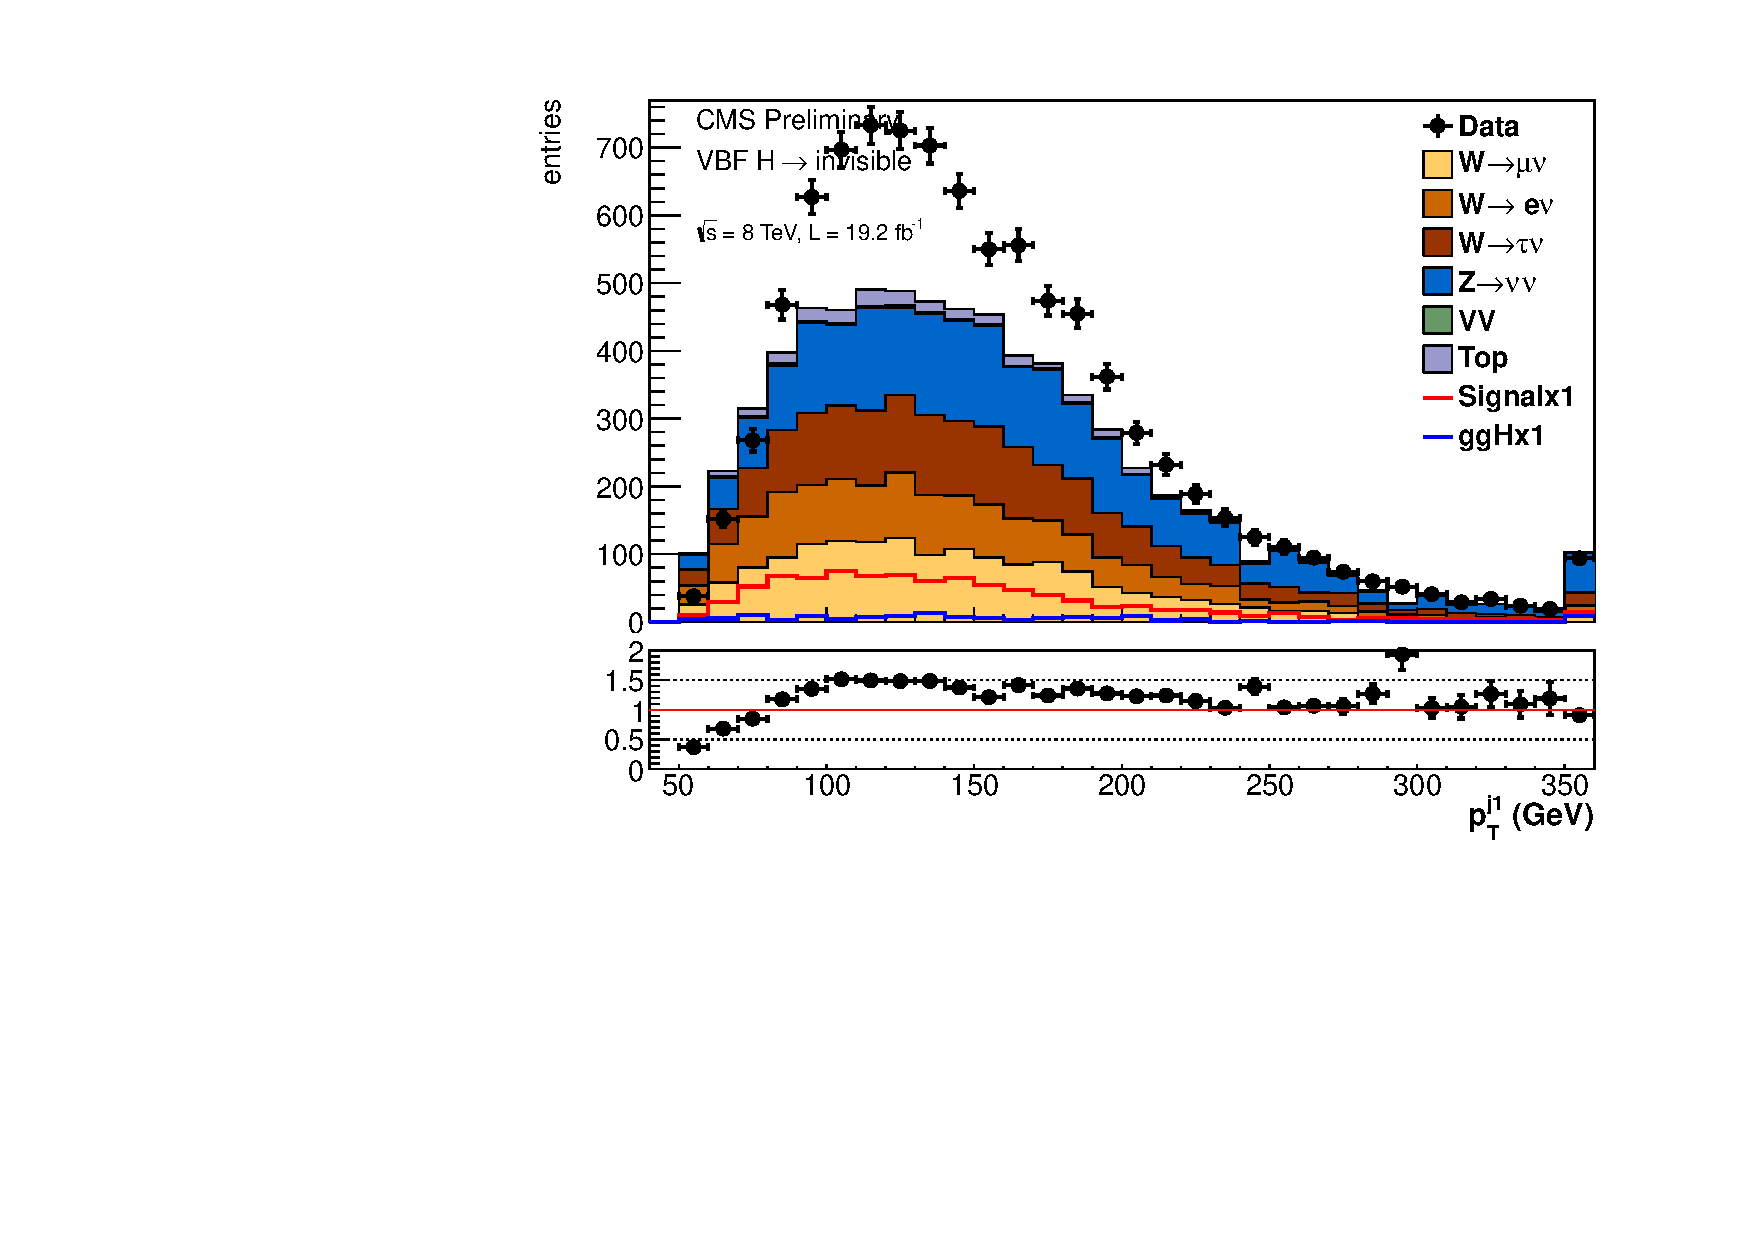
\includegraphics[width=.6\largefigwidth]{plots/parked/AN-14-243-figs/output_presel/nunu_jet1_pt.pdf}
    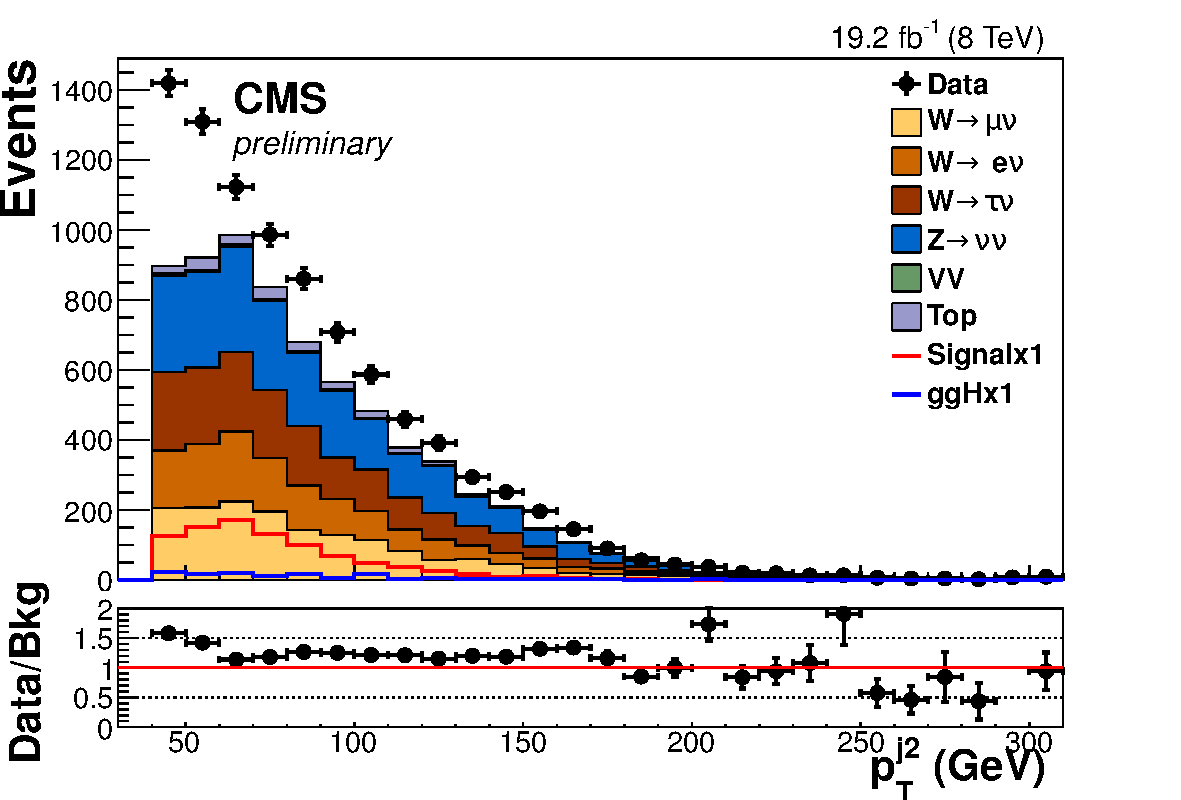
\includegraphics[width=.6\largefigwidth]{plots/parked/AN-14-243-figs/output_presel/nunu_jet2_pt.pdf}

    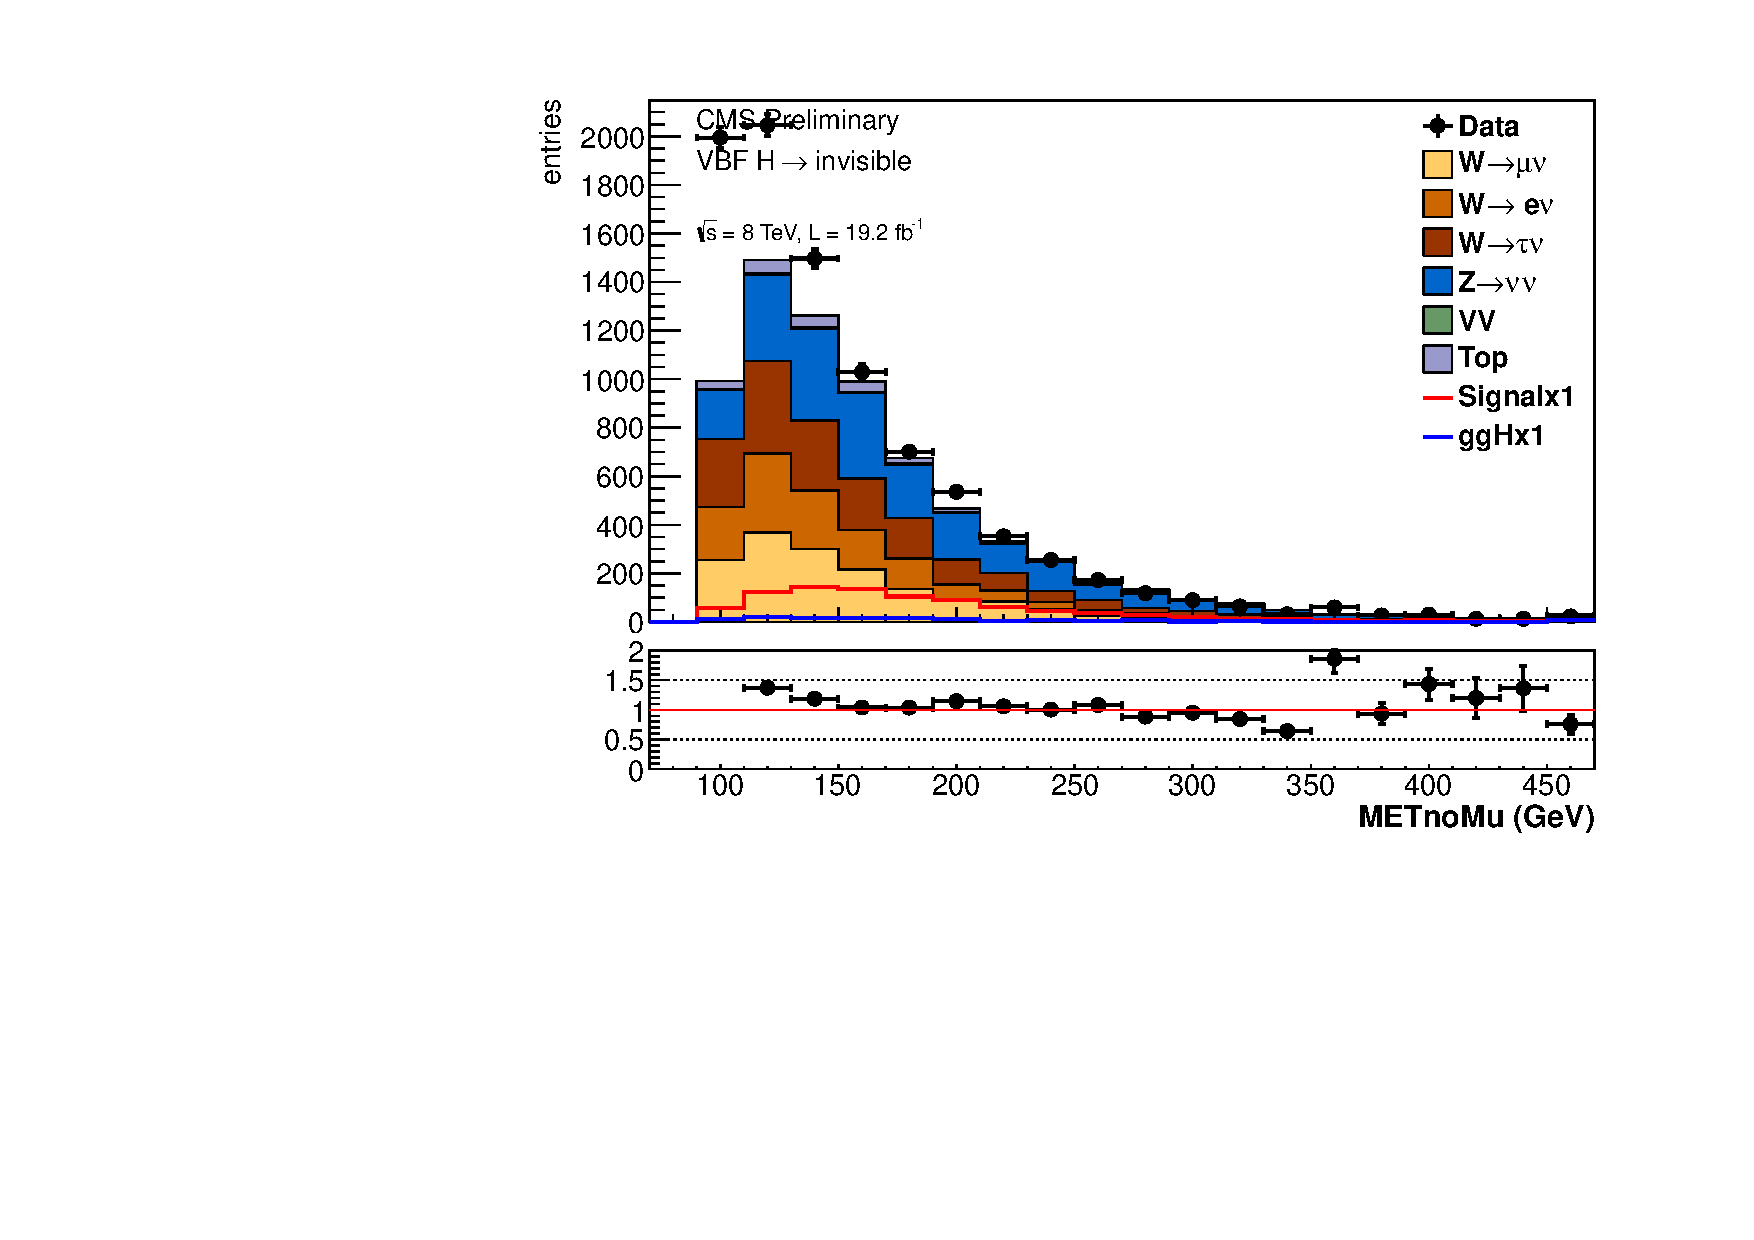
\includegraphics[width=.6\largefigwidth]{plots/parked/AN-14-243-figs/output_presel/nunu_metnomuons.pdf}
    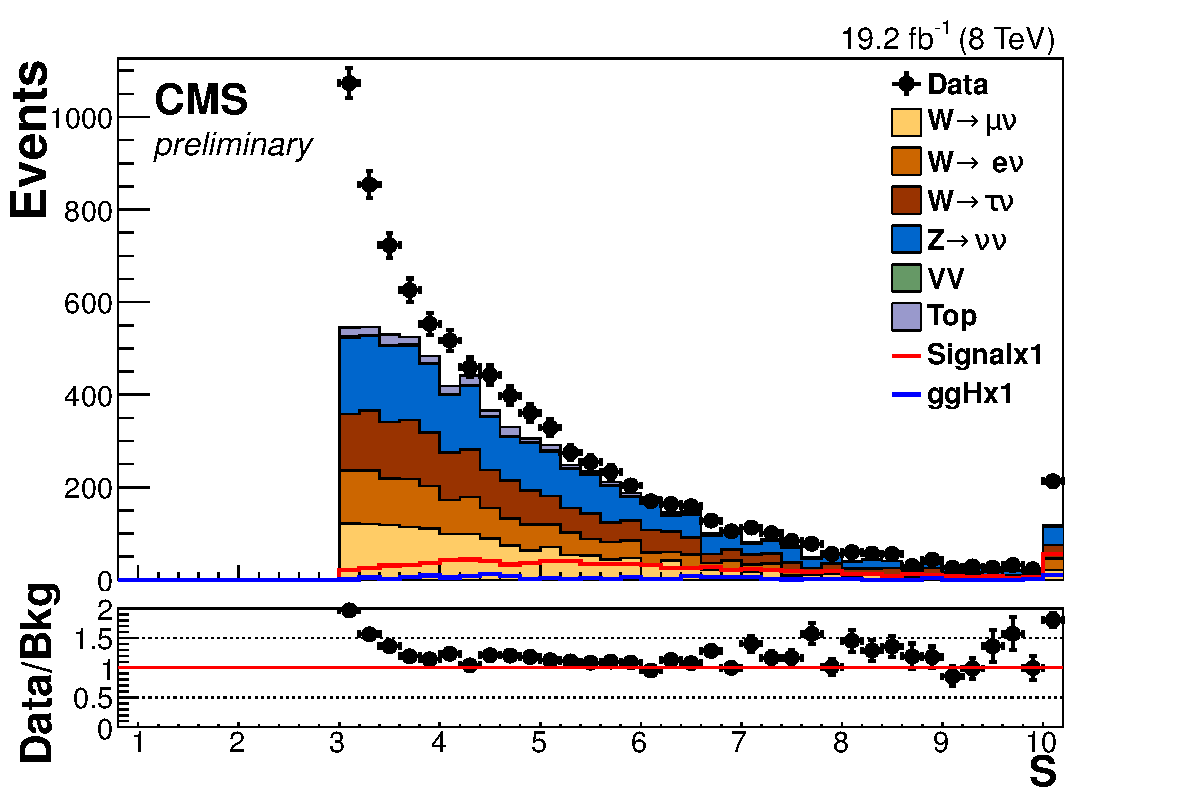
\includegraphics[width=.6\largefigwidth]{plots/parked/AN-14-243-figs/output_presel/nunu_metnomu_significance.pdf}

    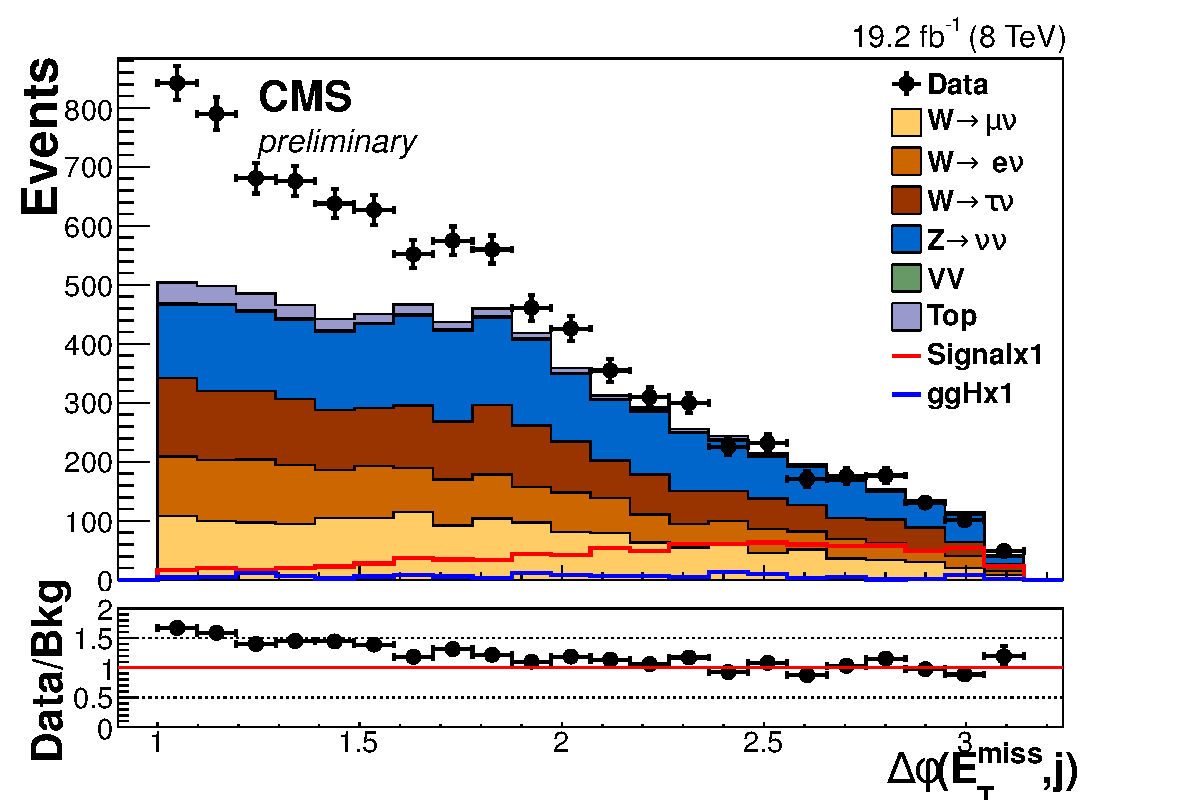
\includegraphics[width=.6\largefigwidth]{plots/parked/AN-14-243-figs/output_presel/nunu_alljetsmetnomu_mindphi.pdf}

  \caption{From top to bottom left to right distributions of \detajj, \Mjj, leading jet \pt, sub-leading jet \pt, \METnoMU, \METsig and \jetmetdphi for events passing the full preselection. No \ac{QCD} multijet contribution is shown, which accounts for the difference between the data observation and background prediction.}
  \label{fig:parkedpostpresel}
\end{figure}





\subsection{Signal region selection}
\label{sec:parkedsigsel}
As can be seen from \FigureRef{fig:parkedpostpresel}, there is still a significant difference between the data and the \ac{MC} background prediction. It is also evident that the main areas where disagreement occurs are where contributions from \ac{QCD} multijet backgrounds (which are not modelled in the figure) would be expected to contribute, i.e. at low \METsig and with jets close to the \METnoMU. Outside these \ac{QCD}-like regions good agreement between data and \ac{MC} is seen. The approach taken was to place tight requirements on these two variables to reduce the \ac{QCD} multijet background to negligible levels, so that it doesn't matter that the uncertainty on the contribution from it is high. A requirement that events have $\jetmetdphi>2$ and $\METsig>4$, was therefore imposed. The resulting relatively \ac{QCD}-free ``optimisation'' region was blinded (i.e. the data were not looked at) to use for studies to determine the final signal region selection.

Two methods of signal region selection were investigated. The first method was a cut based selection. Starting from the optimisation region the cuts on \METsig, \jetmetdphi, \detajj, sub-leading jet \pt and \Mjj were varied one at a time and the expected limit for each cut value was calculated using the method described in \SectionRef{sec:stats} with the background estimation techniques and systematic uncertainties described in Sections~\ref{sec:parkedbkg} and \ref{sec:parkedsyst} respectively. In the case of the \ac{QCD} multijet background, the background estimation was performed once for the optimisation selection and used for all cut values. The estimations for all other background processes were repeated for each set of cuts. After each variable was varied the selection was updated to use the cut value that gave the best expected limit. After all the variables had been varied the process was repeated until no improvement in the expected limit was seen so as to avoid ignoring other better sets of cuts. The cut values that gave the best expected limit define the signal region and are as follows:
\begin{equation}
  \label{eq:parkedsigsel}
  \begin{split}
    \eta_{j1}\cdot\eta_{j2}<0,\detajj>3.6,\,\mathrm{leading\,jet\,\pt}>50 \GeV,\\
    \mathrm{subleading\,jet\,\pt}>45 \GeV, \Mjj>1200 \GeV,\\
    \METnoMU>90 \GeV, \METsig>4.0,\jetmetdphi>2.3.
  \end{split}
\end{equation}
After this selection was defined a second \ac{MVA} based method of optimising the selection was investigated to see if could improve on the cut based selection. \ac{BDT} and fisher %??citation
discriminants were trained using signal and background events passing the signal region selection, and the optimisation procedure defined above was repeated with the value of the discriminant considered as an additional variable. The correlation coefficients between the variables used as inputs to the \ac{MVA} are shown in \FigureRef{fig:parkedmvacorr}. These variables were chosen as they showed the most difference between signal and background distributions and correlations out of a wide range of variables investigated. Without the addition of any additional systematic uncertainties from the understanding of the variables which were input to the \ac{MVA} the best improvement in the expected limit over that of the signal region was less than 1\%. It was therefore decided to use the cut based selection as the final event selection.
\begin{figure}
    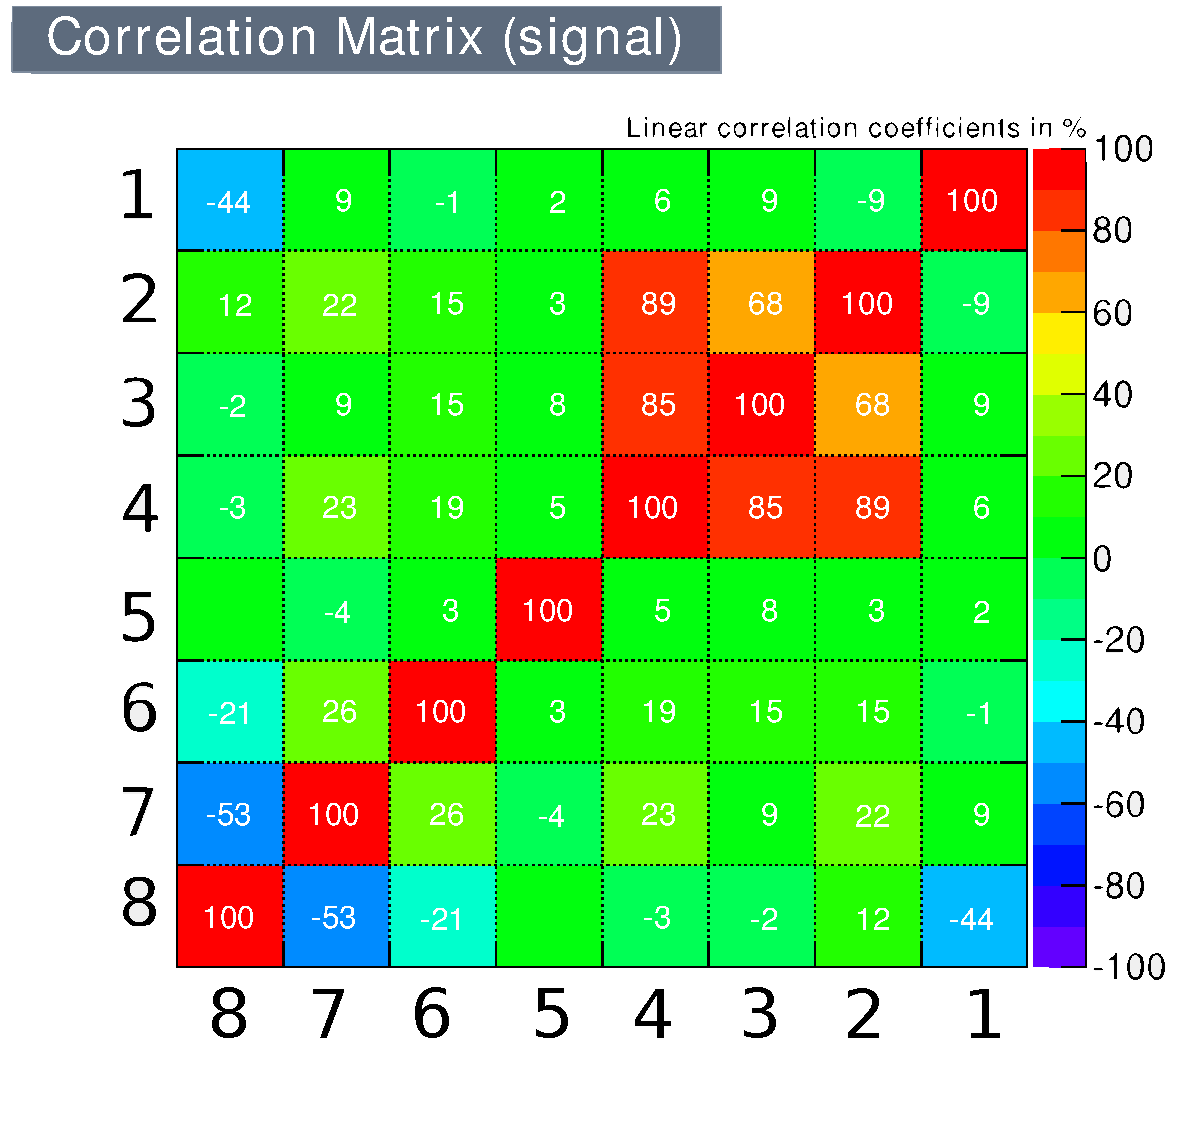
\includegraphics[width=.6\largefigwidth]{plots/parked/AN-14-243-figs/inputcorrsig.pdf}
    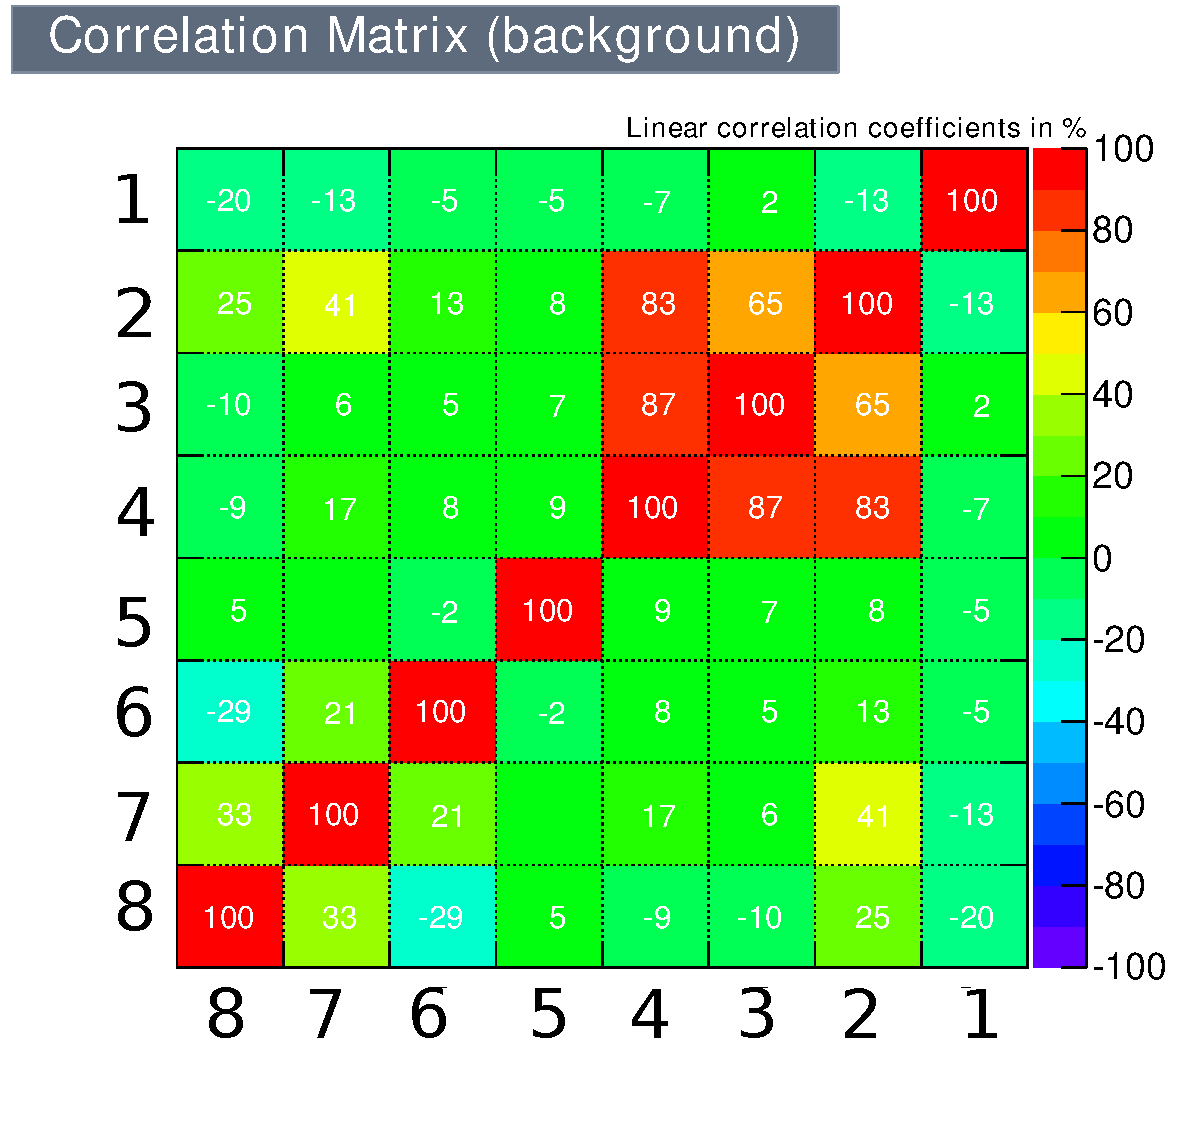
\includegraphics[width=.6\largefigwidth]{plots/parked/AN-14-243-figs/inputcorrbkg.pdf}
  \caption{Matrices of correlation coefficients for several variables in signal (left) and background (right) events passing the signal region selection. The variables are 1) the azimuthal angle difference between the \METnoMU and the unclustered energy in the event, 2) the square root of the hadronic energy in the event, 3) \METsig, 4) \METnoMU, 5) \Mjj, 6) the number of jets with $\pt>30$ \GeV between the two tag jets in \eta, 7) the vectorial sum of the tag jets \pt and the \METnoMU, 8) the ratio between the magnitude of the vectorial sum of the tag jet's \pt and the \METnoMU.}
  \label{fig:parkedmvacorr}
\end{figure}

\section{Background estimation}%??                                                                                                                          
\label{sec:parkedbkg}
The backgrounds contributing to the parked data analysis are the same as those in the prompt data analysis, and the estimation methods used here are also based on those used in the prompt analysis. However, the changes in event selection necessitate several changes from the methods for the prompt analysis. Furthermore, among other improvements, the systematic uncertainty on the \Znunu background was reduced, better understanding of the data driven scale factors was gained and data driven methods of estimating the top quark related background were investigated.

\subsection{Top quarks}%??
Almost all top quarks decay to a \PW boson and a b quark~\cite{pdg}. Top quarks are either created in pairs, in which case there will be two \PW bosons and two b quarks, or via ``single top'' production where only one top quark is created in association with other quarks or a \PW boson and the result is some combination of \PW bosons and quarks. Where at least one of the \PW bosons decays leptonically and the lepton is misreconstructed either of these processes can result in the appearance of \MET and jets that can coincidentally have \ac{VBF}-like topology.
%??smaller than others but worth a go, 
%??two regions, 
%??top vs single top, kinematics different important to get contribution the same as in sig reg
%??top reweighting, 
%??average out to 1 so just use MC

\subsection{W$\rightarrow e\nu$+jets}%??                                                                                                                    
\label{sec:parkedwenu}
The $W\rightarrow e\nu$ background in the parked data analysis is estimated using the same method as 

\subsection{W$\rightarrow \mu\nu$+jets}%??                                                                                                                  
\label{sec:parkedwmunu}

\subsection{W$\rightarrow \tau\nu$+jets}%??                                                                                                                 
\label{sec:parkedwtaunu}

\subsection{Z$\rightarrow \nu\nu$+jets}%??                                                                                                                  
\label{sec:parkedznunu}

\subsection{QCD}%??                                                                                                                                         
\label{sec:parkedQCD}

\subsection{Minor backgrounds}%??
\label{sec:parkedminor}

\section{Systematic uncertainties}%??
\label{sec:parkedsyst}
The uncertainty due to the reweighting process used to account for trigger inefficiencies cancels in all data driven background estimates, as a ratio of \ac{MC} event yields is taken. To estimate the size of the uncertainty that should be applied to processes not taken from data driven background, the bin with the largest uncertainties on its fit for each era was chosen. It was then assumed that all bins had this worst-case uncertainty. This resulted in a 2.3\% overall uncertainty on these processes from this effect. Given that this error is smaller than many of the other errors considered, and that the uncertainty on the efficiency in most of the fit bins is significantly lower than this worst case this uncertainty is considered negligible.



\section{Results}%??                                                                                                                                        
\label{sec:parkedresults}
